% **************************************************
% Document Class Definition
% **************************************************
\documentclass[%
    paper=A4,               % paper size --> A4 is default in Germany
    twoside=true,           % onesite or twoside printing
    openright,              % doublepage cleaning ends up right side
    parskip=half,           % spacing value / method for paragraphs
    chapterprefix=true,     % prefix for chapter marks
    11pt,                   % font size
    headings=normal,        % size of headings
    bibliography=totoc,     % include bib in toc
    listof=totoc,           % include listof entries in toc
    titlepage=on,           % own page for each title page
    captions=tableabove,    % display table captions above the float env
    chapterprefix=false,    % do not display a prefix for chapters
    appendixprefix=false,    % but display a prefix for appendix chapter
    draft=false,            % value for draft version
]{scrreprt}%


% **************************************************
% Setup YOUR thesis document in this file !
% **************************************************
% !TEX root = main.tex


% **************************************************
% Files' Character Encoding
% **************************************************
\PassOptionsToPackage{utf8}{inputenc}
\usepackage{inputenc}


% **************************************************
% Information and Commands for Reuse
% **************************************************
\newcommand{\thesisTitle}{Esercitazione di laboratorio su progetto di cablaggio strutturato e rete locale}
\newcommand{\thesisName}{Riccardo Persello}
\newcommand{\thesisSubject}{Reti di Calcolatori}
\newcommand{\thesisDate}{\today}
\newcommand{\thesisVersion}{1.0}

\newcommand{\thesisFirstSupervisor}{Pier Luca Montessoro}

\newcommand{\thesisUniversity}{\protect{Università degli Studi di Udine}}
\newcommand{\thesisUniversityDepartment}{Dipartimento di Ingegneria e Architettura}
\newcommand{\thesisUniversityGroup}{Corso di Ingegneria Elettronica}


% **************************************************
% Debug LaTeX Information
% **************************************************
%\listfiles


% **************************************************
% Load and Configure Packages
% **************************************************
\usepackage[italian]{babel} % babel system, adjust the language of the content
\PassOptionsToPackage{% setup clean thesis style
    figuresep=colon,%
    hangfigurecaption=false,%
    hangsection=true,%
    hangsubsection=true,%
    sansserif=false,%
    configurelistings=true,%
    colorize=full,%
    colortheme=bluemagenta,%
    configurebiblatex=true,%
    bibsys=biber,%
    quotesstyle=italian,%
    bibfile=bibliography,%
    bibstyle=numeric,%
    bibsorting=nty,%
}{cleanthesis}
\usepackage{cleanthesis}

\hypersetup{% setup the hyperref-package options
    pdftitle={\thesisTitle},    %   - title (PDF meta)
    pdfsubject={\thesisSubject},%   - subject (PDF meta)
    pdfauthor={\thesisName},    %   - author (PDF meta)
    plainpages=false,           %   -
    colorlinks=false,           %   - colorize links?
    pdfborder={0 0 0},          %   -
    breaklinks=true,            %   - allow line break inside links
    bookmarksnumbered=true,     %
    bookmarksopen=true          %
}

\bibliography{bib-refs}
\renewcommand\lstlistlistingname{Elenco dei listati}

\usepackage{siunitx}
\sisetup{detect-all}


% **************************************************
% Document CONTENT
% **************************************************
\begin{document}

% uncomment the following command to fill up pages with
% whitespace instead of aligning the first and last lines
% of a page (see \raggedbottom vs. \flushbottom)
%\raggedbottom

% --------------------------
% rename document parts
% --------------------------
%\renewcaptionname{ngerman}{\figurename}{Abb.}
%\renewcaptionname{ngerman}{\tablename}{Tab.}
%\renewcaptionname{english}{\figurename}{Fig.}
%\renewcaptionname{english}{\tablename}{Tab.}
\renewcaptionname{italian}{\figurename}{Fig.}
\renewcaptionname{italian}{\tablename}{Tab.}

% --------------------------
% Front matter
% --------------------------
\pagenumbering{roman}			% roman page numbing (invisible for empty page style)
\pagestyle{empty}				% no header or footers
% !TEX root = ../my-thesis.tex
%
% ------------------------------------  --> cover title page
\begin{titlepage}
	\pdfbookmark[0]{Cover}{Cover}
	\flushright\hfill
	\vfill
	{\LARGE\thesisTitle\par}
	\rule[5pt]{\textwidth}{.4pt} \par
	{\Large\thesisName}
	\vfill
	\textit{\large\thesisDate} \\
	% Version: \thesisVersion
\end{titlepage}


% ------------------------------------  --> main title page
\begin{titlepage}
	\pdfbookmark[0]{Titlepage}{Titlepage}
	\tgherosfont\centering

	% {\Large \thesisUniversity} \\[4mm]
	
\includegraphics[width=6cm]{gfx/uniud.jpeg} \\[2mm]
	\textsf{\thesisUniversityDepartment} \\
	\textsf{\thesisUniversityGroup} \\

	\vfill
	{\large \thesisSubject} \\[5mm]
	{\LARGE \color{ctcolortitle}\textbf{\thesisTitle} \\[10mm]}
	{\Large \thesisName} \\

	\vfill

	\normalfont\flushleft{
		\small
		\textbf{\thesisName}\\
		\textit{\thesisTitle}\\
		\thesisSubject, \thesisDate\\
		Docente: \thesisFirstSupervisor\\[1.5em]
		\textbf{\thesisUniversity}\\
		\thesisUniversityDepartment\\
		\thesisUniversityGroup\\
	}
\end{titlepage}
		% INCLUDE: all titlepages
\cleardoublepage{}

\pagestyle{plain}				% display just page numbers
% !TEX root = ../my-thesis.tex
%
\pdfbookmark[0]{Abstract}{Abstract}
\addchap*{Abstract}
\label{sec:abstract}

\blindtext

\vspace*{20mm}

{\usekomafont{chapter}Abstract (different language)}
\label{sec:abstract-diff}

\blindtext
		% INCLUDE: the abstracts (english and german)
\cleardoublepage{}
%
% % !TEX root = ../my-thesis.tex
%
\pdfbookmark[0]{Acknowledgement}{Acknowledgement}
\addchap*{Acknowledgement}
\label{sec:acknowledgement}

\Blindtext[2][2]
 % INCLUDE: acknowledgement
% \cleardoublepage{}
%
\currentpdfbookmark{\contentsname}{toc}
\setcounter{tocdepth}{2}		% define depth of toc
\tableofcontents				% display table of contents
\cleardoublepage{}

% --------------------------
% Body matter
% --------------------------
\pagenumbering{arabic}			% arabic page numbering
\setcounter{page}{1}			% set page counter
\pagestyle{scrheadings}			% header and footer style

%% Uncomment the following lines using the \part command
%% to add part sections
% \part{Example Part}
% !TEX root = ../../../main.tex
%

\chapter{Cablaggio Strutturato}
Inserire descrizione.     % INCLUDE: 1 - introduction
% !TEX root = ../../../main.tex
%

\section{Analisi}
Prima di procedere con la prima parte del progetto, è necessario analizzare collettivamente
le planimetrie ed i requisiti indicati. Si sceglie di iniziare dai requisiti necessari a soddisfare
gli utenti finali di questo progetto, ovvero i dipendenti aziendali (ed in genere chiunque debba collegarsi
alla rete in questione). Dal punto di vista del cablaggio strutturato, il vincolo è dato principalmente dalle
postazioni e dalle apparecchiature da collegare alla rete cablata, in quanto richiederanno un numero minimo
ben preciso di prese a muro necessarie a garantire il loro collegamento assieme ad una ridondanza
sufficientemente elevata. Questo si rivela utile al fine di scongiurare interventi eccessivamente lunghi,
costosi ed invasivi nell'eventualità del danneggiamento di una linea od un apparato di rete.

\subsection{Conteggio delle prese utente}         % INCLUDE: 1 - analysis
% !TEX root = ../../../main.tex
%

\newpage
\section{Progettazione}
\subsection{Tipo di presa}

\begin{wrapfigure}{r}{5cm}
  \centering
  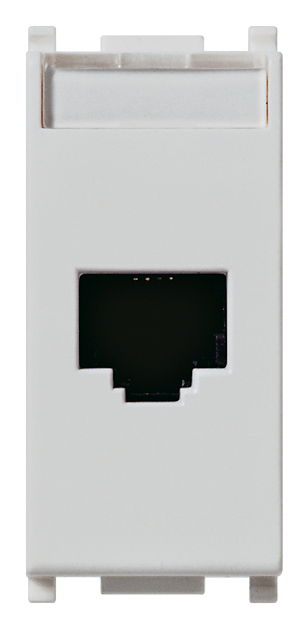
\includegraphics{vimar-14338-8-SL.jpg}
  \caption{Il connettore scelto per le prese utente.}\label{fig:presa}
\end{wrapfigure}

Supponendo che l'edificio abbia già alcune scatole elettriche incassate dedicate all'impianto di rete,
dove necessarie (anche condivise con altri connettori/controlli), non si terrà conto del costo di queste ultime.

Si sceglie di utilizzare prodotti di marca Vimar, serie Netsafe.
Nello specifico, si sceglie di usare dei connettori RJ45 Cat5e UTP (codice 14338.8.SL), illustrato in figura~\ref{fig:presa}.

Dato che determinate scatole elettriche possono contenere anche prese, pulsanti, interruttori o altri tipi
di dispositivi, non si conosce la dimensione (e di conseguenza il costo) delle placche decorative e dei supporti di montaggio.

Si suppone pertanto di affidarsi a quanto già predisposto per l'impianto elettrico (ove possibile).

Notare che nella maggior parte dei casi, questo non sarà necessario, in quanto gran parte dell'impianto,
per motivi di flessibilità e semplicità, verrà posato a pavimento, con delle prese direttamente disponibili sulle scrivanie.

Nei casi in cui è invece necessario affidarsi a delle prese a muro, resta valido quanto prima descritto.

\subsection{Dislocazione degli armadi e dorsale principale}

Data la topografia stellare del cablaggio orizzontale, si preferisce ospitare gli armadi per la \textit{floor distribution}
nei locali tecnici centrali all'edificio, in ogni piano. Essendo già stato fissato dalla planimetria fornita, il centralino
telefonico sarà per forza posizionato nel locale tecnico sud-ovest del piano terreno, assieme alle apparecchiature per
il collegamento alla rete pubblica.

Con questa scelta, il server (posizionato al piano terreno), godrà di una distanza ridotta con l'armadio di piano, garantendo
un miglior collegamento (in quanto si assume che il server necessiti di una considerevole quantità di banda), ed una maggiore
flessibilità nel caso in cui, in futuro, dovessero essere necessarie delle espansioni.

I collegamenti di dorsale dell'edificio saranno inizialmente orizzontali, dirette dal locale tecnico sud-ovest del piano terreno
verso quello centrale. Da quel punto, si muoveranno in verticale, raggiungendo gli altri armadi. La stessa cosa vale per i collegamenti
addizionali tra armadi adiacenti.

\subsection{Cablaggio orizzontale}

Si suppone di avere a disposizione un sistema di cablaggio a pavimento galleggiante, comprensivo di più canalette di larghezza sufficientemente
ampia da poter accogliere complessivamente, nelle parti iniziali del percorso, circa la metà di tutti i cavi utilizzati nel cablaggio di un singolo piano.

Per quanto concerne la sala riunioni, essendo adiacente al locale tecnico contenente l'armadio, ed essendo dotata di numerose prese,
si preferisce evitare di dover passare il cablaggio attraverso il corridoio: si preferisce attraversare il muro, predisposto con
un foro di diametro sufficiente, per raggiungere i tavoli da sotto il pavimento. Qui, le connessioni saranno poste al centro del tavolo principale
e su quello del presentatore mediante delle scatole elettriche oblique da scrivania.

Si ritiene utile sfruttare un passaggio simile per il raggiungimento della vicina sala server e, per i piani superiori,
del corridoio al lato opposto della porta presente nel locale tecnico. Non si ritiene ragionevole il percorrimento a ``U'' del corridoio
principale per il solo fine di raggiungere degli uffici altrimenti molto vicini in linea d'aria.

Queste considerazioni sono riportate nelle planimetrie che seguono (figure~\ref{fig:planimetria-terreno-cablaggio}~e~\ref{fig:planimetria-1-cablaggio}). I cablaggi di dorsale sono tracciati con delle linee
di spessore maggiore, ed i cerchi indicano il passaggio tra piani differenti.

Gli armadi sono evidenziati in azzurro e le prese in fuchsia.

Il cablaggio si distingue nel seguente modo:
\begin{description}
  \item[Verde] Fibra ottica multimodale 50/125.
  \item[Arancione] Cavi in rame Cat5e per Ethernet.
  \item[Rosso] Cavi in rame voice-grade (Cat3) per fonia.
\end{description}

\begin{figure}[ht]
  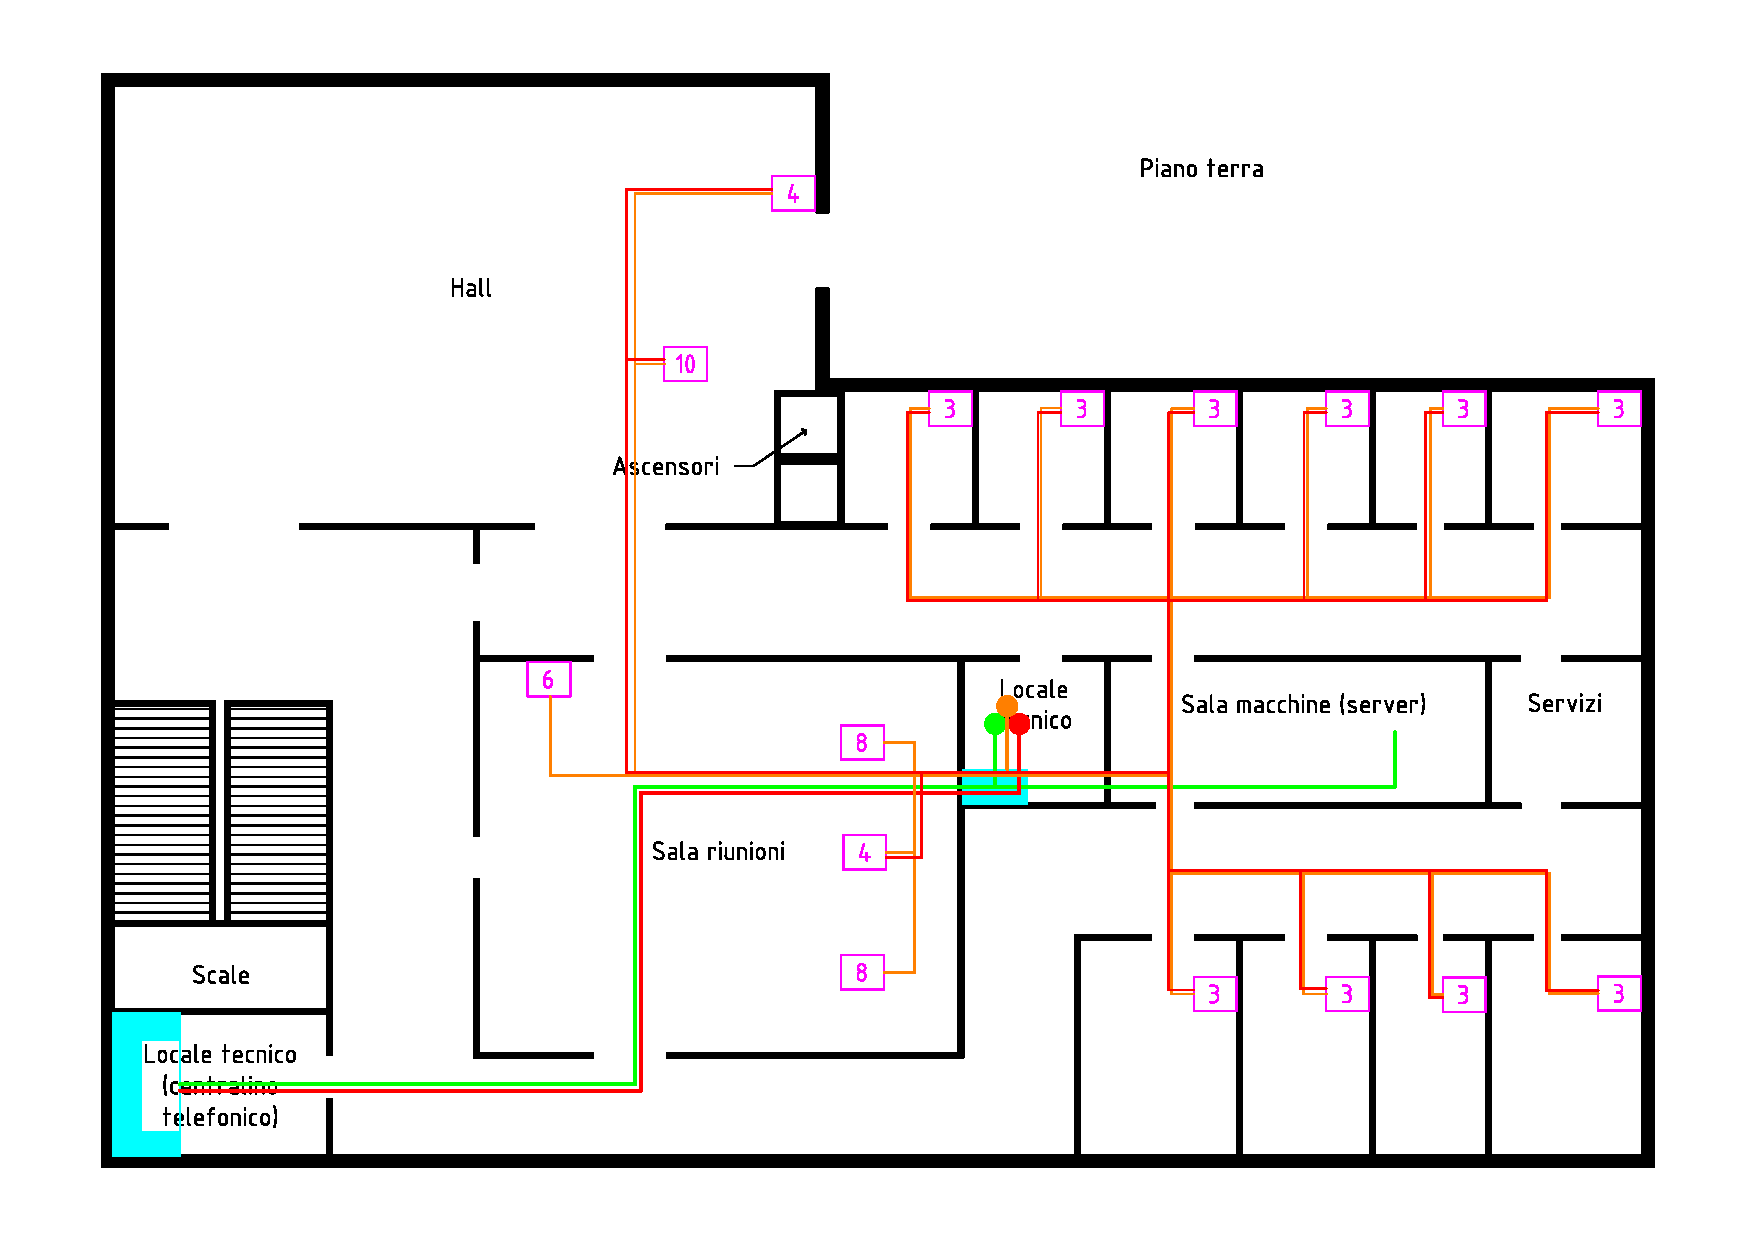
\includegraphics[angle=90,origin=c,width=\textwidth]{planimetrie-pianoterra-cablaggio}
  \caption{Cablaggio del piano terreno.}\label{fig:planimetria-terreno-cablaggio}
\end{figure}

\begin{figure}[ht]
  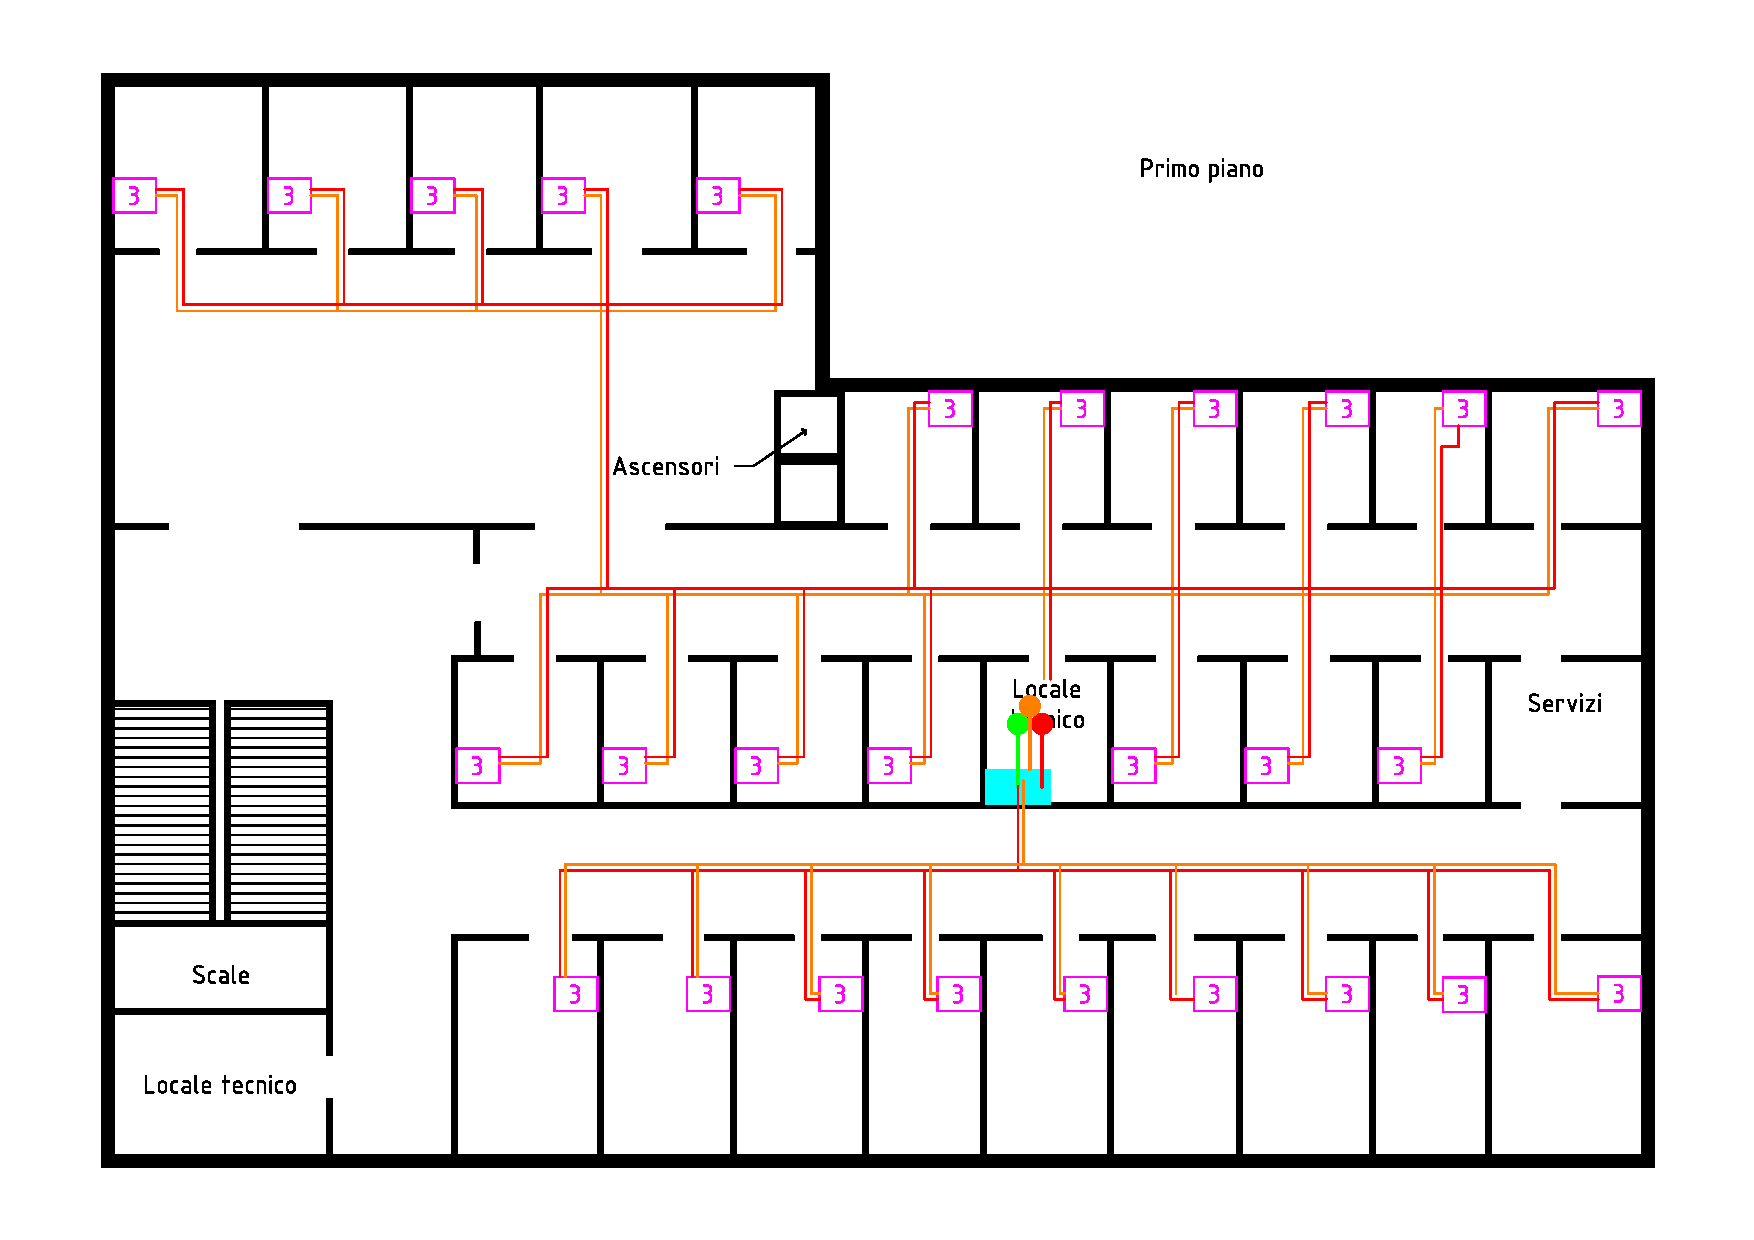
\includegraphics[angle=90,origin=c,width=\textwidth]{planimetrie-piano1-cablaggio}
  \caption{Cablaggio dei piani da primo a quarto.}\label{fig:planimetria-1-cablaggio}
\end{figure}

Si contano due pareti attraversate nel piano terra, e soltanto una per piano nei superiori.
          % INCLUDE: 1 - project
% !TEX root = ../../../main.tex
%

\newpage
\section{Elenco dei materiali}

L'elenco dei materiali è consultabile alla figura~\ref{fig:elenco-materiali}, a fine capitolo, dopo le planimetrie.

Il costo parziale dei materiali è di 18546,72€.

Si procede ora con la seconda parte del progetto, riguardante l'infrastruttura di rete locale.

\begin{figure}[ht]
  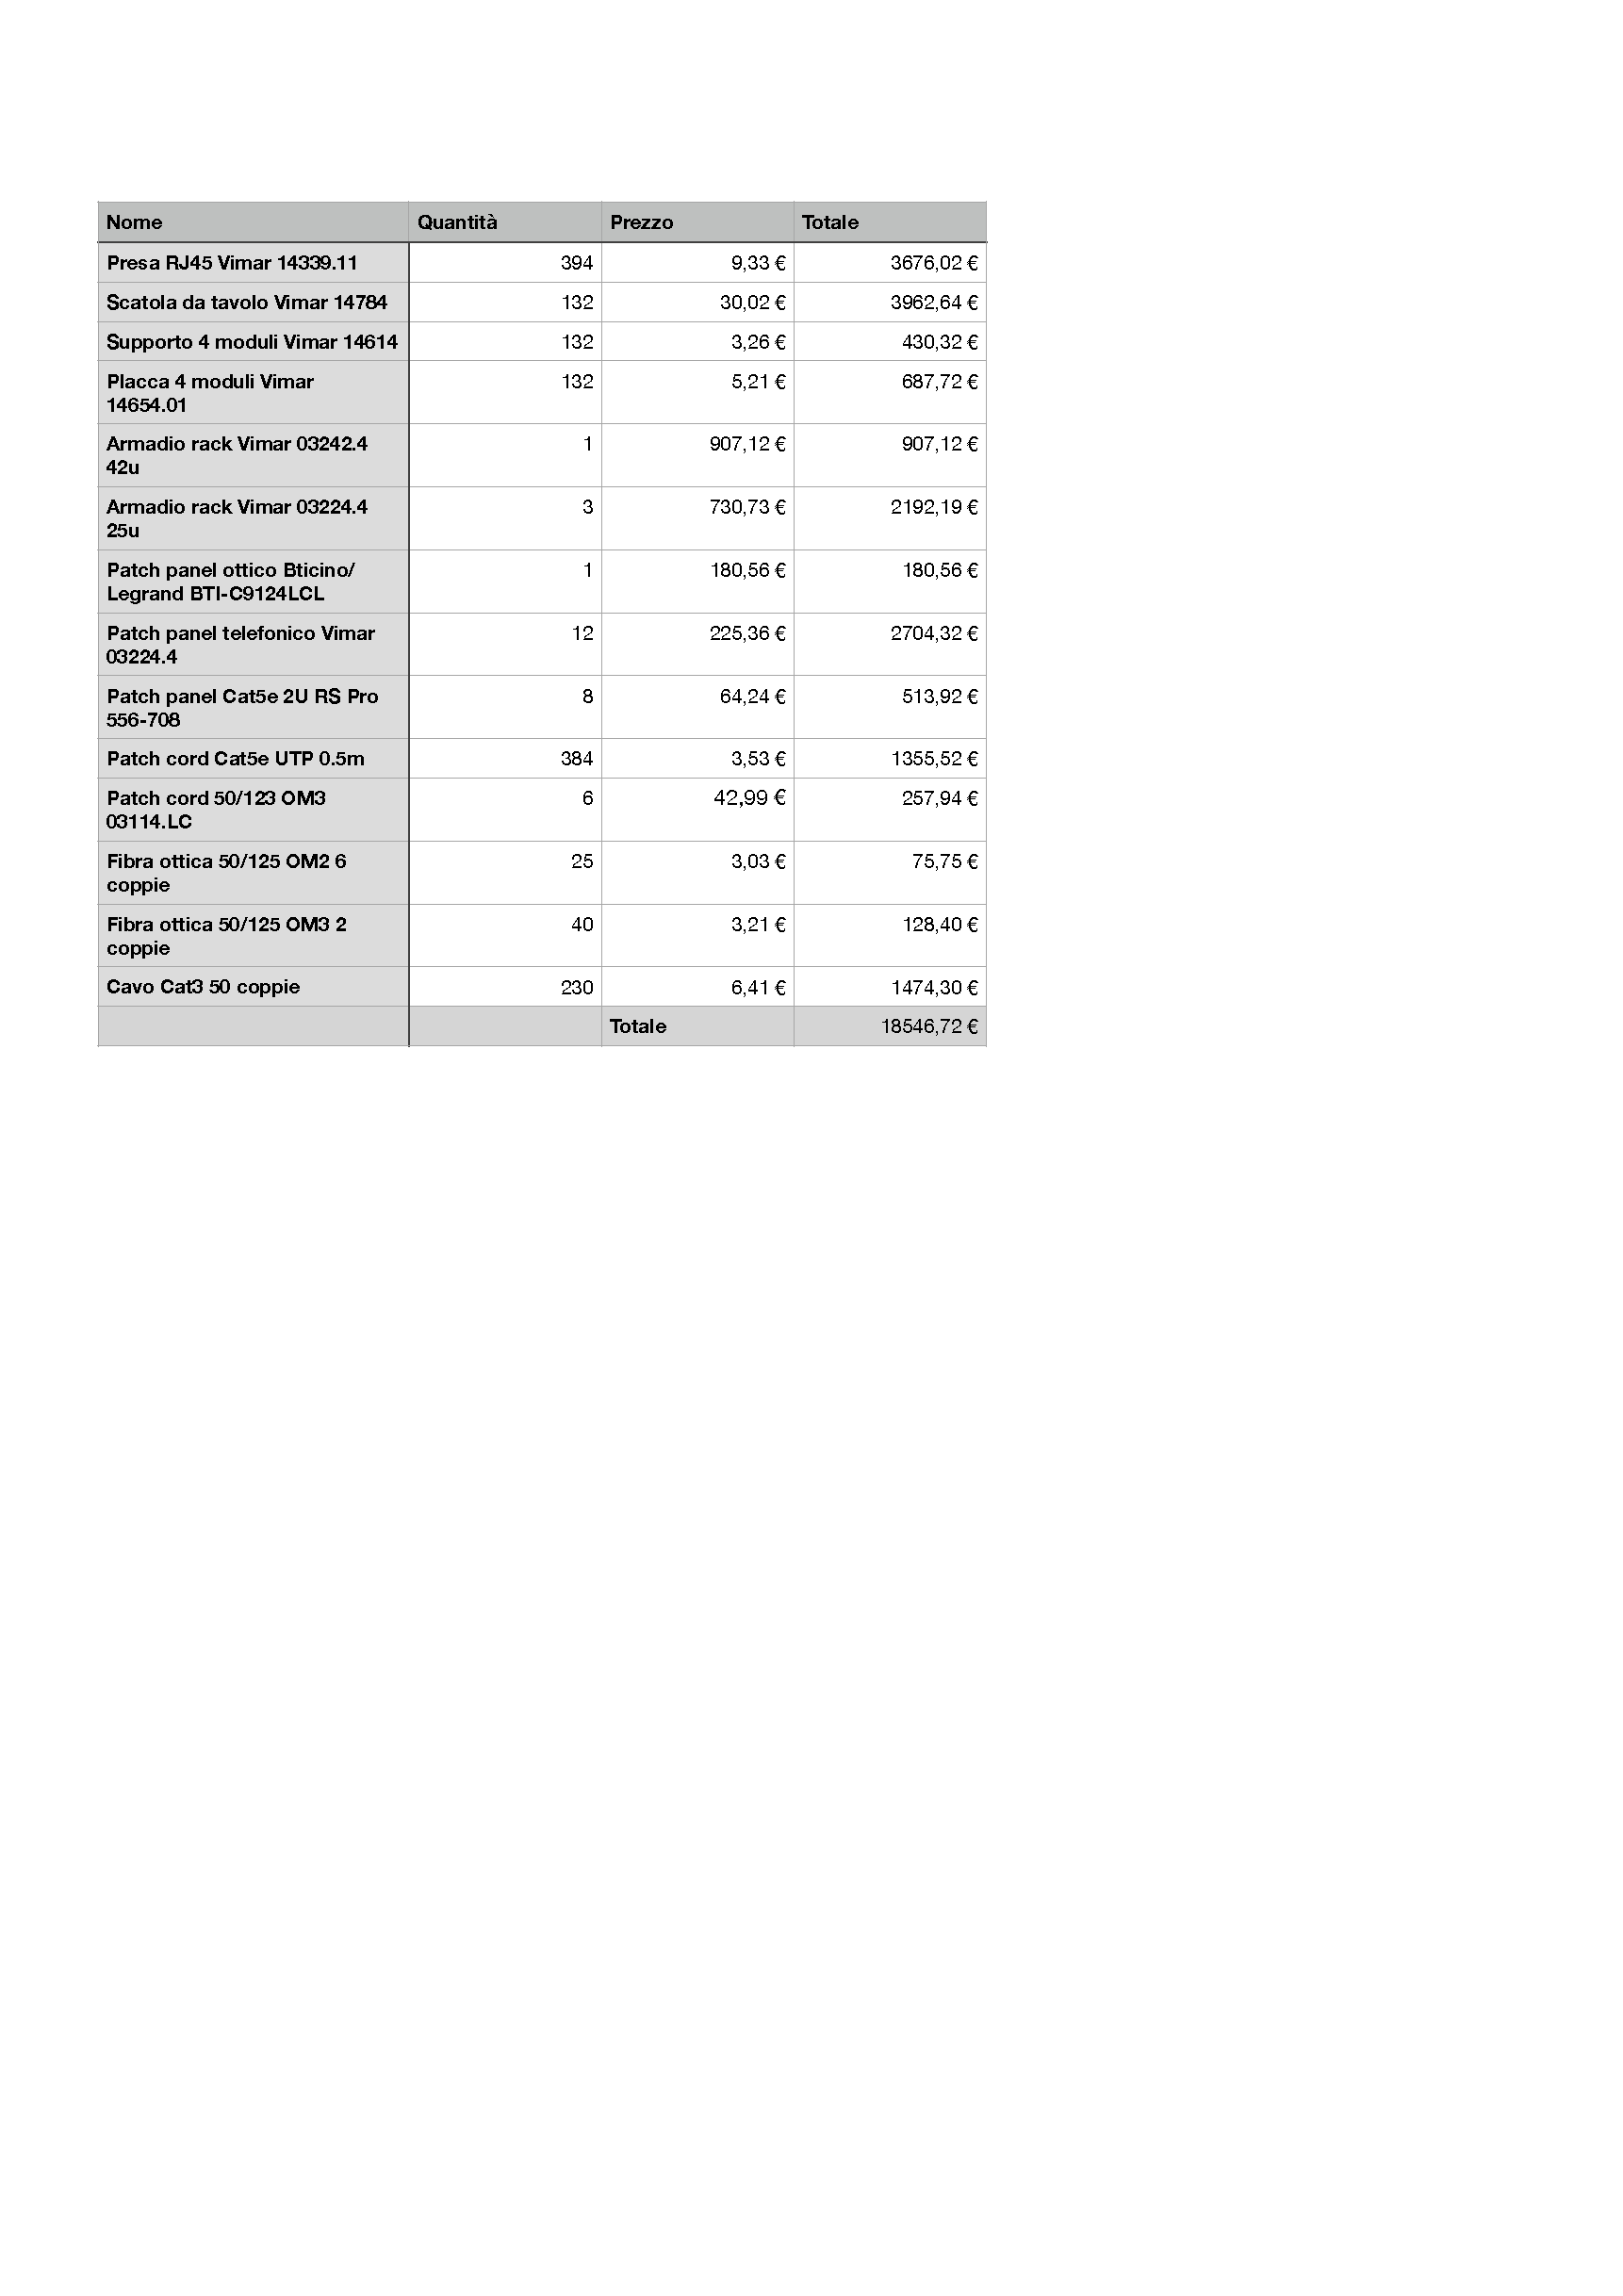
\includegraphics[width=\textwidth]{BOM-1}
  \caption{Tabella dei materiali necessari per il cablaggio}\label{fig:elenco-materiali}
\end{figure}       % INCLUDE: 1 - conclusion
% !TEX root = ../../../main.tex

\chapter{Rete locale}

\section{Planimetrie}
Si riportano di seguito le planimetrie dei vari piani,comprendenti le informazioni necessarie
a stabilire la suddivisione delle postazioni di lavoro nelle relative sottoreti.

\begin{figure}[ht]
  \centering
  \begin{minipage}{.5\textwidth}
    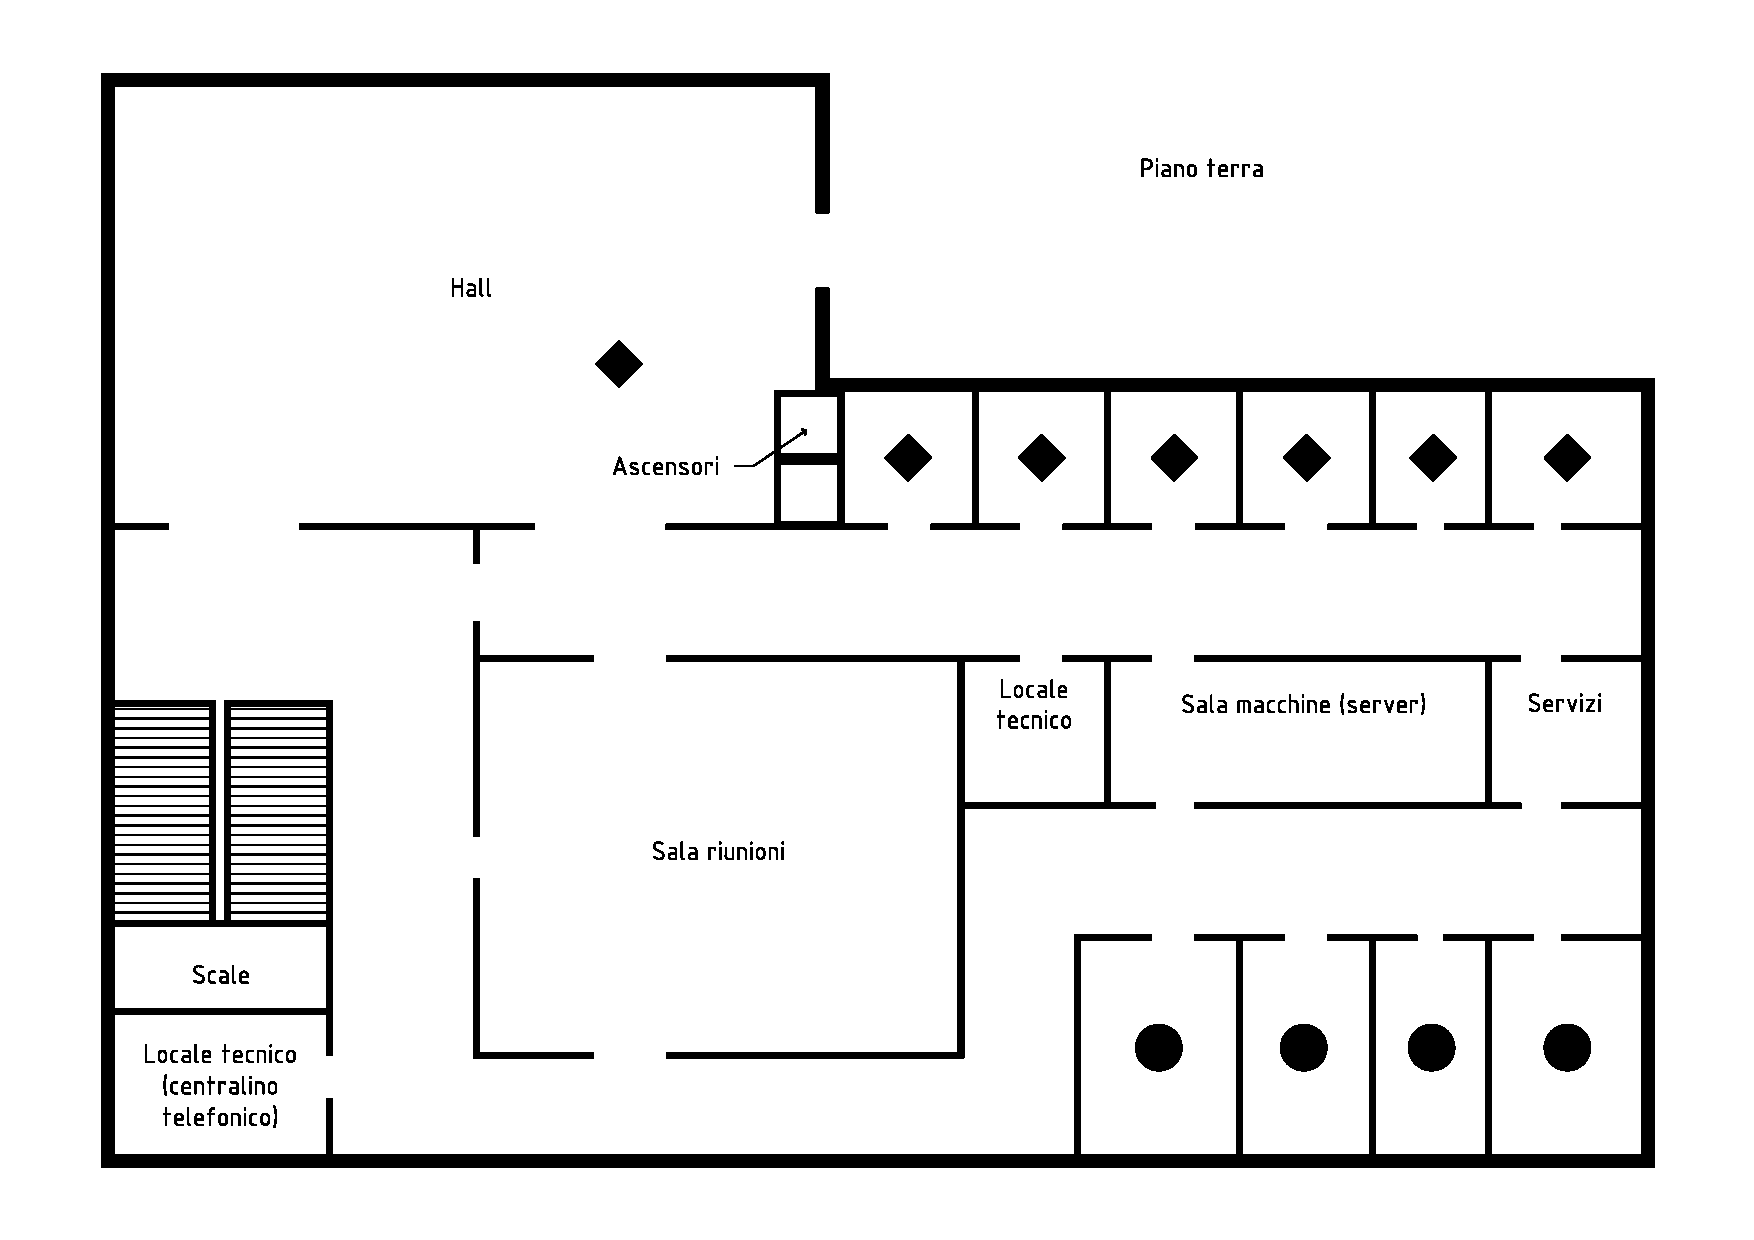
\includegraphics[width=\textwidth]{planimetrie-pianoterra-utenze}
  \end{minipage}%
  \begin{minipage}{.5\textwidth}
    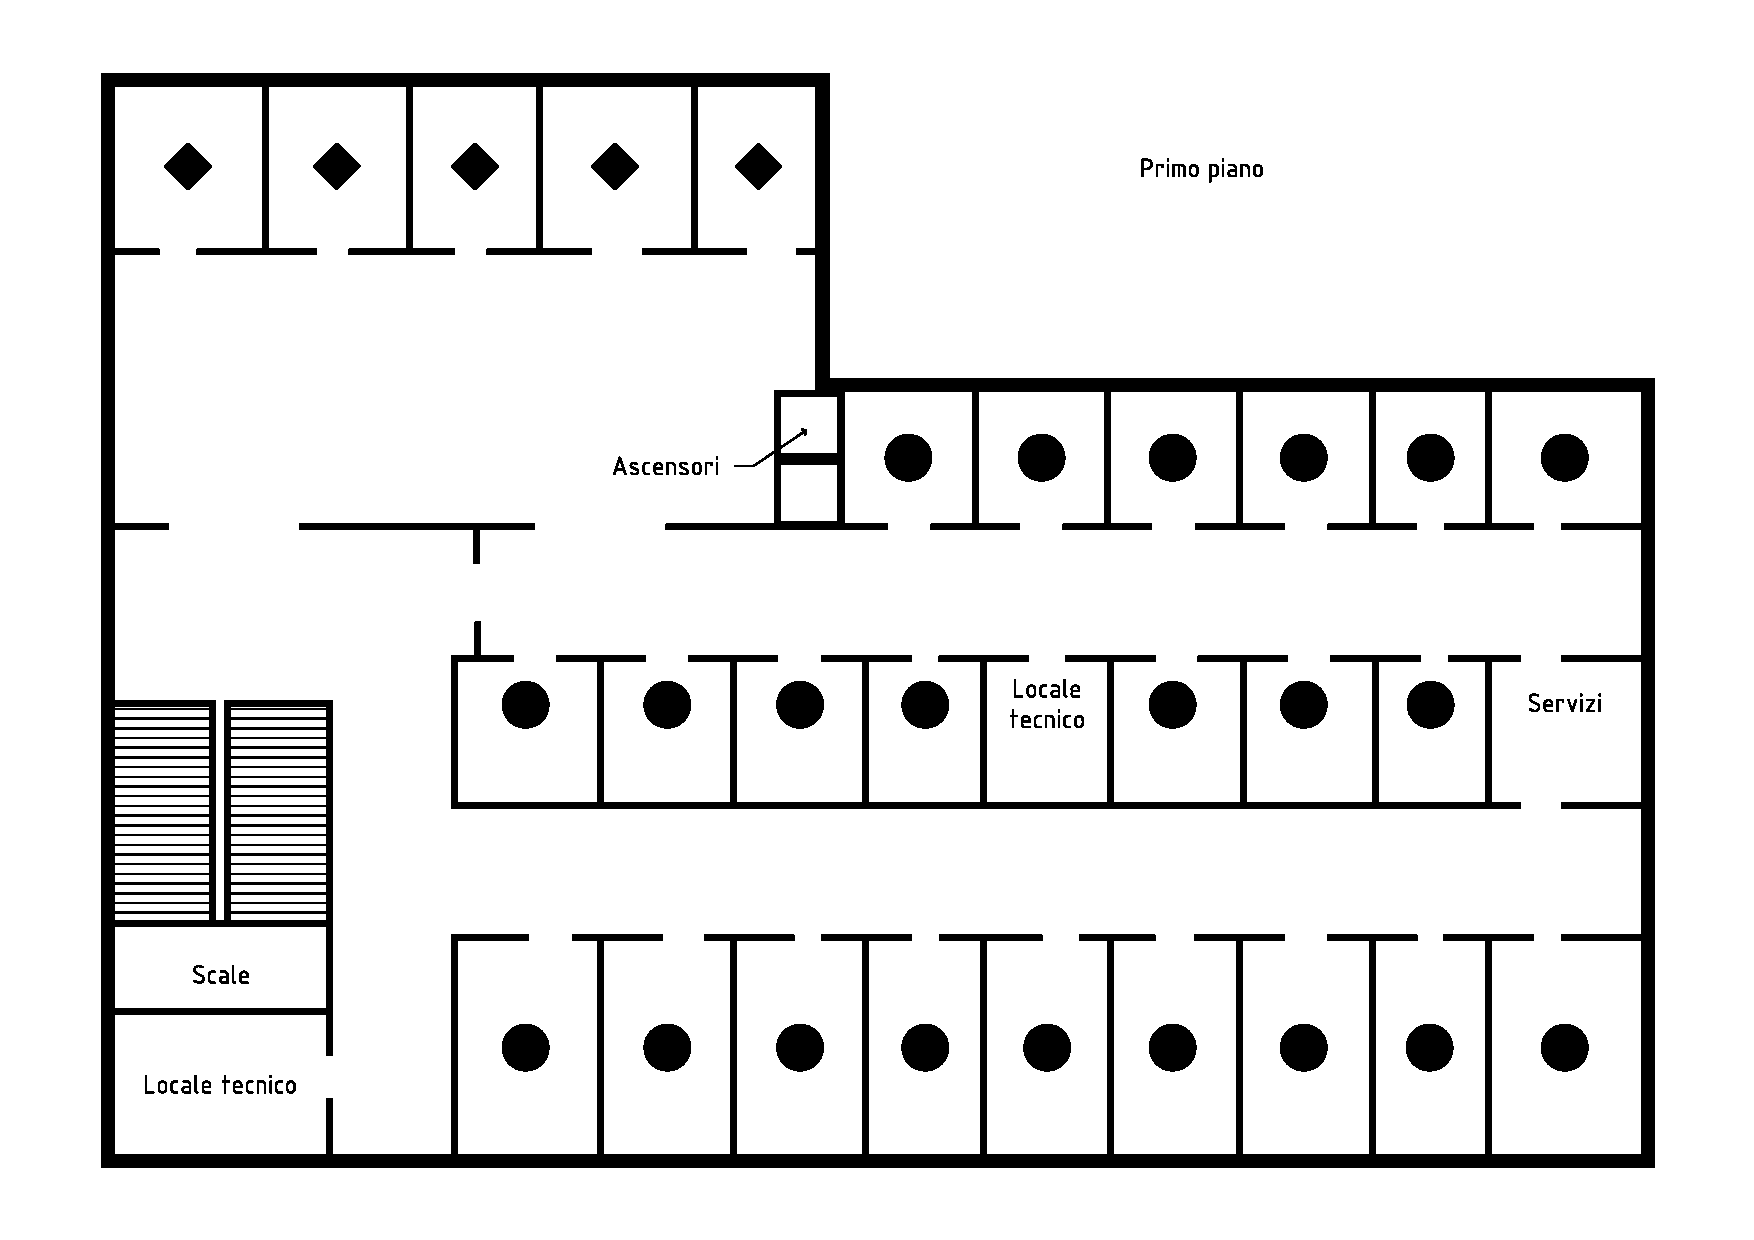
\includegraphics[width=\textwidth]{planimetrie-piano1-utenze}
  \end{minipage}
  \begin{minipage}{.5\textwidth}
    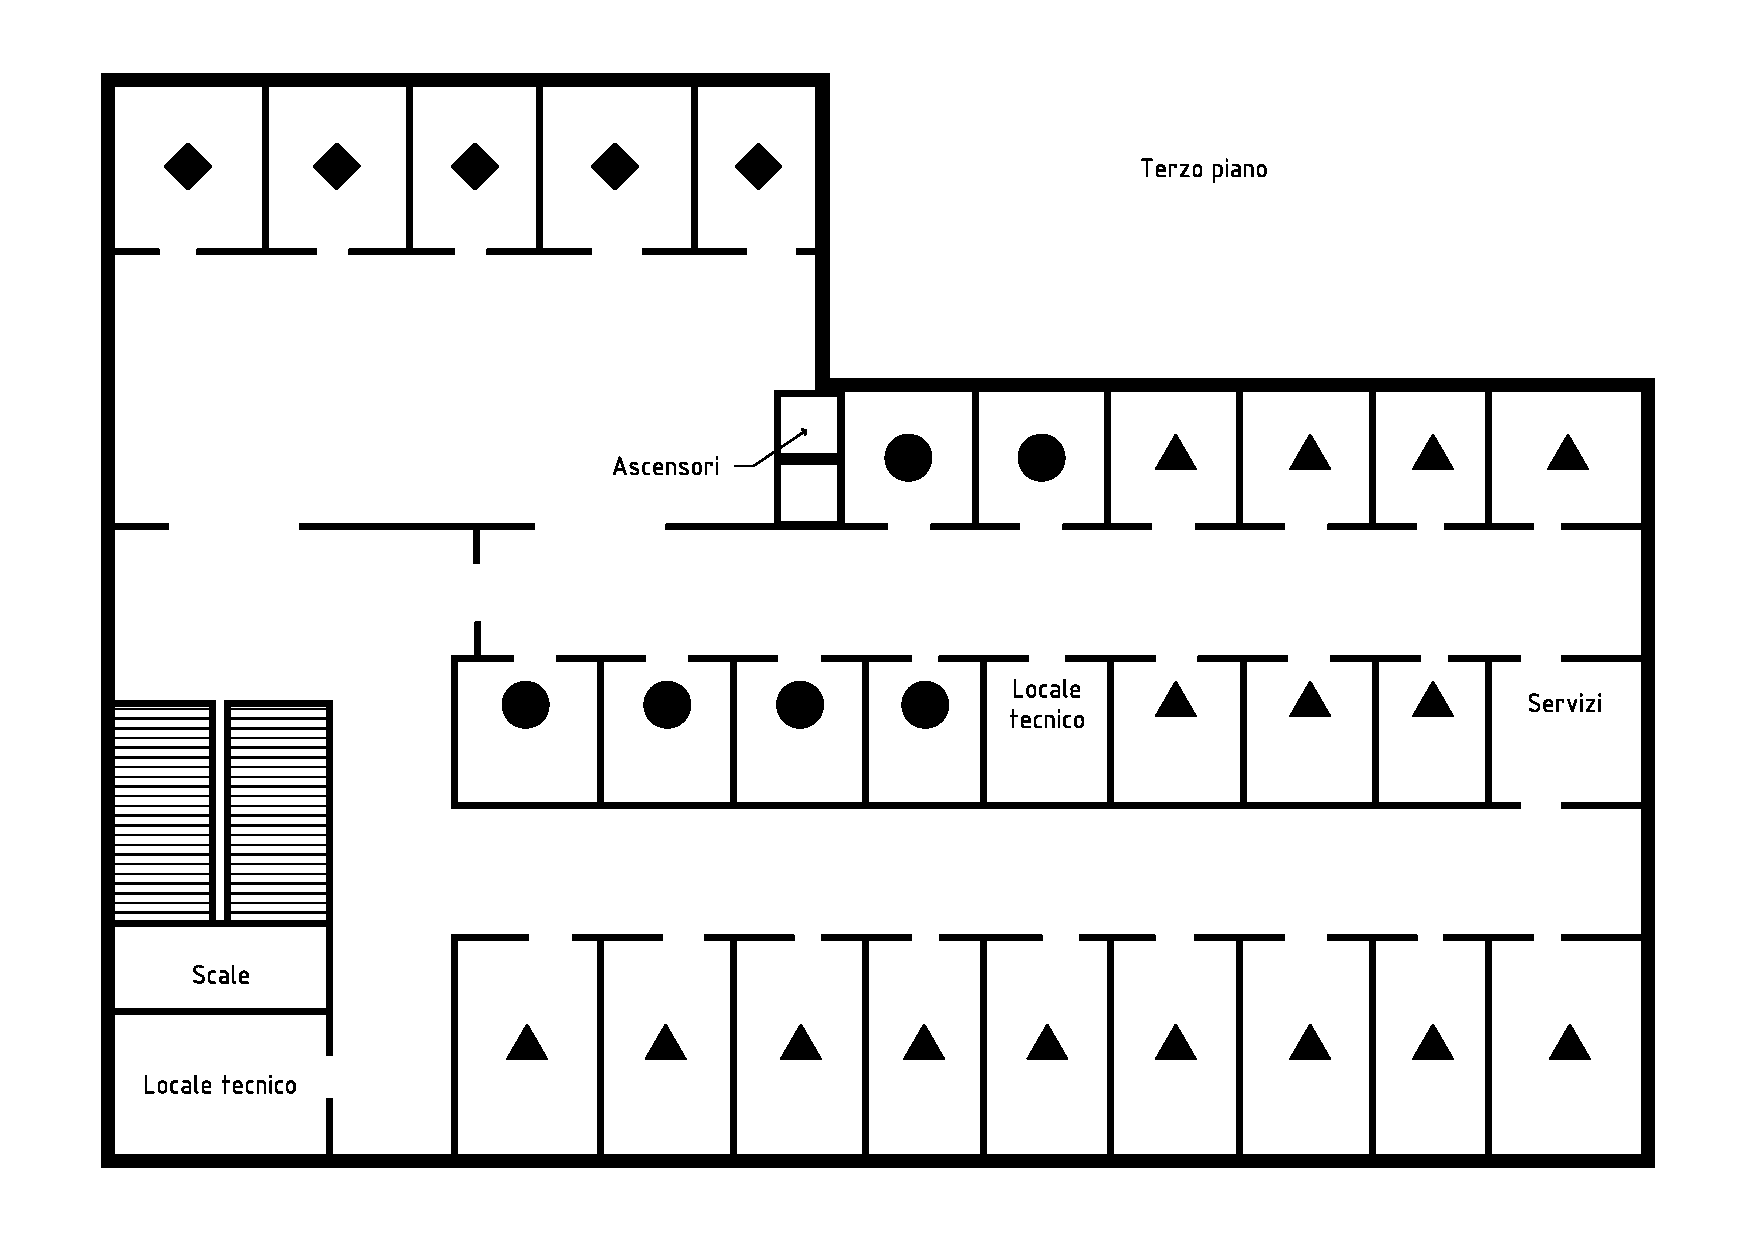
\includegraphics[width=\textwidth]{planimetrie-piano3-utenze}
  \end{minipage}
  \caption{Planimetrie con utenze.}\label{fig:planimetrie-utenze}
\end{figure}

\newpage
\section{Le sottoreti}
Ci sono tre sottoreti: la LAN di amministrazione, comprendente 28 postazioni, quella di produzione,
con 56 postazioni, ed infine quella sperimentale, da 32 utenze.

Si ritiene necessario, per motivi di sicurezza, associare alcuni dispositivi ad una rete completamente separata
rispetto a queste tre, ovvero tutti i punti in cui ci può essere un accesso condiviso ad informazioni sensibili.
Si ritiene pertanto utile isolare tutte le prese di rete presenti sul tavolo della sala riunioni insieme agli access point
per un'eventuale rete wireless per coloro che sono esterni all'azienda, in modo che, anche durante una riunione con
clienti o personale esterno (ma anche tra gruppi interni ma separati dell'azienda), non ci siano rischi per la sicurezza
delle informazioni che viaggiano sulle reti locali.

Per garantire una maggiore flessibilità a questi gruppi, si sceglie di utilizzare dispositivi di rete in grado
di creare reti LAN virtuali (VLAN).     % INCLUDE: 2 - introduction
% !TEX root = ../../../main.tex

\section{Dispositivi di rete}
Si sceglie, per la successiva semplicità di gestione ed una maggiore integrazione, di utilizzare dispositivi dello
stesso produttore. In particolare, si utilizzeranno dispositivi Ubiquiti UniFi.

\subsection{Centro stella}
Al centro stella, troviamo due dispositivi principali.

Il primo, il \textit{Dream Machine Pro}, è un dispositivo multiuso. Consente innanzitutto di gestire
l'intera rete, essendo una console per gli altri dispositivi in rete. Integra inoltre funzionalità di sicurezza
ed offre otto connessioni Ethernet che potrebbero essere utili per vari usi: essendo il primo dispositivo connesso
alla rete esterna, possono essere utilizzate per quelle apparecchiature che devono garantire una maggiore stabilità
nella connessione, come un server web o un sistema antifurto. In questo modo, anche se un dispositivo al di sotto
di questo fallisce, la connessione resterà attiva.

Per migliorare la stabilità della rete, utile in caso di fallimento completo della dorsale ottica, è possibile connettere
il \textit{floor distributor} del piano terreno a quattro delle porte disponibili su questo dispositivo mediante
collegamenti Ethernet Cat5e, prolungando la linea di backup.

Successivamente, connesso in cascata a questo dispositivo mediante una bretella ottica, vi è un sistema di \textit{Switch Aggregation},
ovvero uno switch di livello 2 per fibra ottica con 8 porte SFP+ da 10 Gb/s. Da questo partono le ramificazioni verso i vari \textit{floor
  distributor}.

\subsection{Floor distributor}
Ogni floor distributor sarà dotato, oltre ai dispositivi definiti nella sezione di cablaggio strutturato,
di uno \textit{Switch Pro 48}, uno switch di livello 3 dotato di 48 porte Ethernet e quattro porte SFP+.

Vista l'abbondanza di porte adatte al collegamento in fibra ottica, invece di eliminare le parti di fibra
in eccesso durante il cablaggio (si ricorda che ci sarà un cavo da 6 coppie, di cui 4 in uso, percorrente
l'intero edificio in verticale), le si potrebbero utilizzare per la creazione di un'altra linea di backup,
equivalente a quella realizzata mediante i quattro collegamenti tra armadi adiacenti. Se la rete è
configurata adeguatamente, questo aiuterebbe parecchio il traffico interno, in quanto non sarà necessario
l'attraversamento dello switch ``ottico''. Visto che molti software e sistemi operativi offrono funzionalità
di caching, una simile infrastruttura di rete aumenterebbe le performance quando vi è la necessità di installare
o aggiornare software su tutti i dispositivi aziendali, riducendo degli eventuali tempi morti.

Saranno necessari degli adattatori SFP con collegamento LC. Anche questi sono disponibili dallo stesso produttore
delle altre apparecchiature di rete.

La topologia generale è descritta dalla figura~\ref{fig:topologia}.

\newpage
\section{Resoconto}

\begin{table}[ht]
  \begin{tabular}{@{}lcrr@{}}
    \toprule
    Nome              & Tipo di dispositivo          & Quantità & Prezzo totale \\ \midrule
    Dream Machine Pro & Console/Router (L3)/Firewall & 1        & 319.00€       \\ \midrule
    Switch Pro 48     & Router (L3)                  & 5        & 2495.00€      \\ \midrule
    Switch Aggregator & Switch (L2), ottico          & 1        & 229.00€       \\ \midrule
    UF-MM-1G-20       & Adattatori SFP+              & 20       & 119.00€       \\ \bottomrule
  \end{tabular}
  \caption{Resoconto sugli apparati di rete attivi.}\label{tab:apparati-rete}
\end{table}

Come da tabella~\ref{tab:apparati-rete}, grazie alla flessibilità delle VLAN, non è necessario
l'uso di una grande quantità di dispositivi. Il subtotale per questa sezione ammonta a 3162€, IVA esclusa.
I prezzi sono stati trovati sullo store europeo di Ubiquiti. Non si includono nel conteggio eventuali
apparecchiature wireless, facilmente incorporabili.

\begin{figure}[ht]
  \centering
  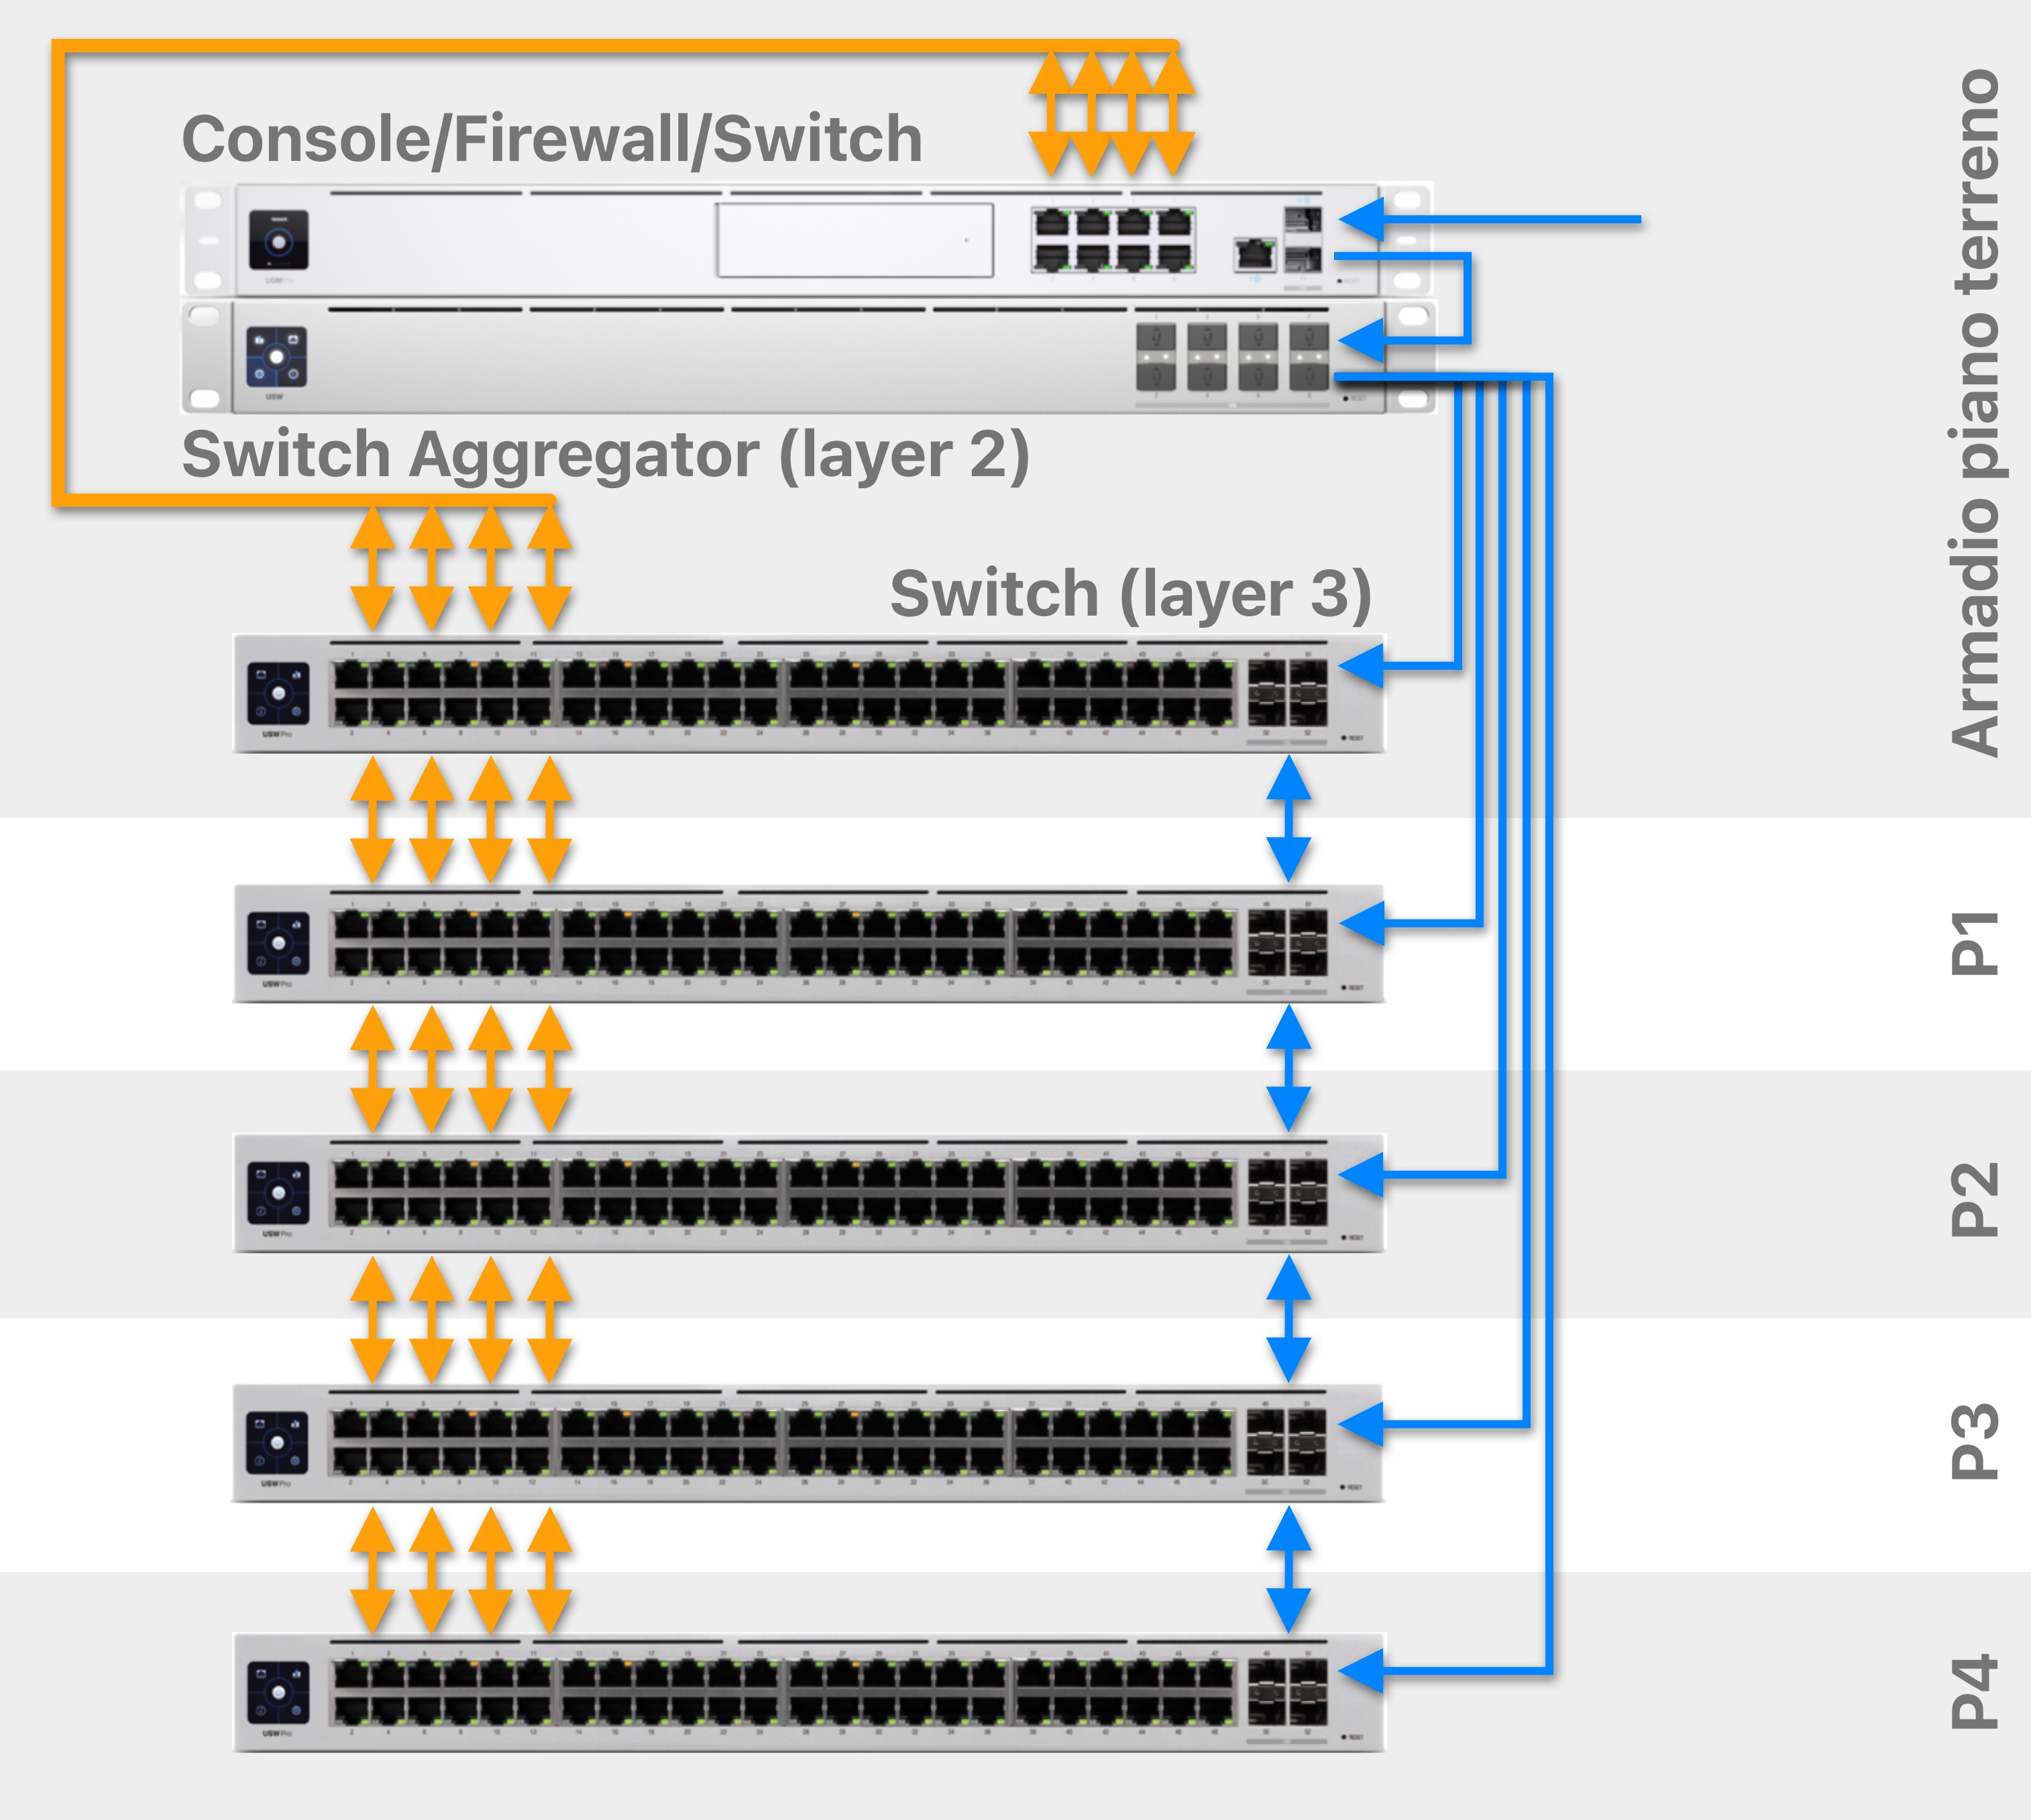
\includegraphics[height=10cm]{struttura-rete.jpg}
  \caption{
    Topologia della rete: in arancione, connessioni Ethernet su cavo Cat5e, in blu, quelle su fibra ottica multimodale. %
    Non tutte le connessioni sono obbligatorie, alcune sono ridondanti.
  }\label{fig:topologia}
\end{figure}

\newpage
\subsection{Considerazioni sulla tolleranza ai guasti}
La rottura di un router comporta la chiusura dei collegamenti di tutto il piano, ed interrompe anche
le linee di backup. Eventuali connessioni interne dovranno passare per lo switch a fibra ottica.

La rottura di uno dei due apparecchi di centro stella (o del collegamento con l'esterno) non inibisce la
comunicazione interna. Come prima specificato, è ottimale connettere le apparecchiature più importanti per l'accesso
esterno direttamente alla console (gateway), la quale ha funzionalità di switch di livello 3 su 8 prese Ethernet RJ45.

Anche se lo switch per fibra ottica dovesse smettere di funzionare, grazie all'estensione della linea di backup,
gli uffici manterranno comunque la connessone ad Internet, probabilmente con prestazioni ridotte.

Il fallimento della console principale (gateway) o della linea in fibra ottica, comporta la caduta della connessione Internet.
In generale, si ritiene difficile la totale interruzione del servizio intranet. 

Questi sistemi garantiscono inoltre, mediante l'acquisto di dispositivi aggiuntivi, una eventuale linea di backup
su rete LTE. Una simile soluzione potrebbe essere utile a mantenere attivi alcuni servizi essenziali (con ovvie limitazioni di velocità)
anche durante disservizi sulla linea fissa.
          % INCLUDE: 2 - project
% !TEX root = ../../../main.tex

\chapter{Piano di indirizzamento IP}

\section{VLAN}
I dispositivi scelti hanno dei preset per la creazione di VLAN. Nello specifico, per le tre reti
richieste, si utilizzerà un preset di tipo ``Corporate'', il quale consente la comunicazione tra
reti virtuali differenti. Si potrà successivamente creare una rete di tipo ``Guest'' isolata da queste.

La console consente la gestione di queste reti virtuali mediante un'interfaccia grafica in cui si
possono configurare gli switch presenti, porta per porta. Inoltre, nonostante venga teoricamente effettuato in maniera
automatica, è possibile assegnare un range di indirizzi IP per ogni VLAN, divisi per router.

Per la rete ``Guest'' si porrà un numero di indirizzi fissi assegnabili alle prese del tavolo
della sala riunioni, ma non sapendo il numero di utenti connessi alla futura rete WLAN, si consiglia di
impostare gli access point con degli indirizzi pubblici, ma effettuanti NAT per tutti i dispositivi a loro connessi.

Se si desidera visualizzare una simulazione della schermata di configurazione di un sistema simile,
visitare il sito \url{demo.ui.com}. La creazione di nuove reti virtuali è disponibile nella parte di
impostazioni accessibili dall'icona in basso a sinistra, nella sezione ``Networks''.

\begin{table}[ht]
  \begin{adjustbox}{center}
    \begin{tabular}{@{}lll@{}}
      \toprule
      Subnet             & Range                     & Utilizzo                  \\ \midrule
      196.111.250.0/26   & \begin{tabular}[c]{@{}l@{}}196.111.250.1 - 196.111.250.62\\ 196.111.250.63 Broadcast\end{tabular} & \begin{tabular}[c]{@{}l@{}}Riservata per la gestione della rete.\\Una parte di questa subnet\\(isolata con mod. Guest)\\sarà dedicata collegamento ospiti.\end{tabular} \\
      196.111.250.64/26  & \begin{tabular}[c]{@{}l@{}}196.111.250.65 - 196.111.250.126\\ 196.111.250.127 Broadcast\end{tabular} & LAN amministrazione       \\
      196.111.250.128/26 & \begin{tabular}[c]{@{}l@{}}196.111.250.129 - 196.111.250.190\\ 196.111.250.191 Broadcast\end{tabular} & LAN produzione            \\
      196.111.250.192/26 & \begin{tabular}[c]{@{}l@{}}196.111.250.193 - 196.111.250.254\\ 196.111.250.255 Broadcast\end{tabular} & LAN sperimentale          \\ \bottomrule
    \end{tabular}
  \end{adjustbox}
  \caption{Il piano di indirizzamento generale.}\label{tab:piano-ind-generale}
\end{table}

\newpage
\subsection{Subnetting}
Dato che è stato specificato un numero massimo di 62 indirizzi pubblici per subnet, si sceglie di
utilizzare una netmask da 26 bit. In questo modo, 2 bit identificheranno il numero di rete ed altri
6 saranno disponibili per 64 indirizzi IP.

Nello specifico, fare riferimento al seguente schema:

\begin{figure}[ht]
  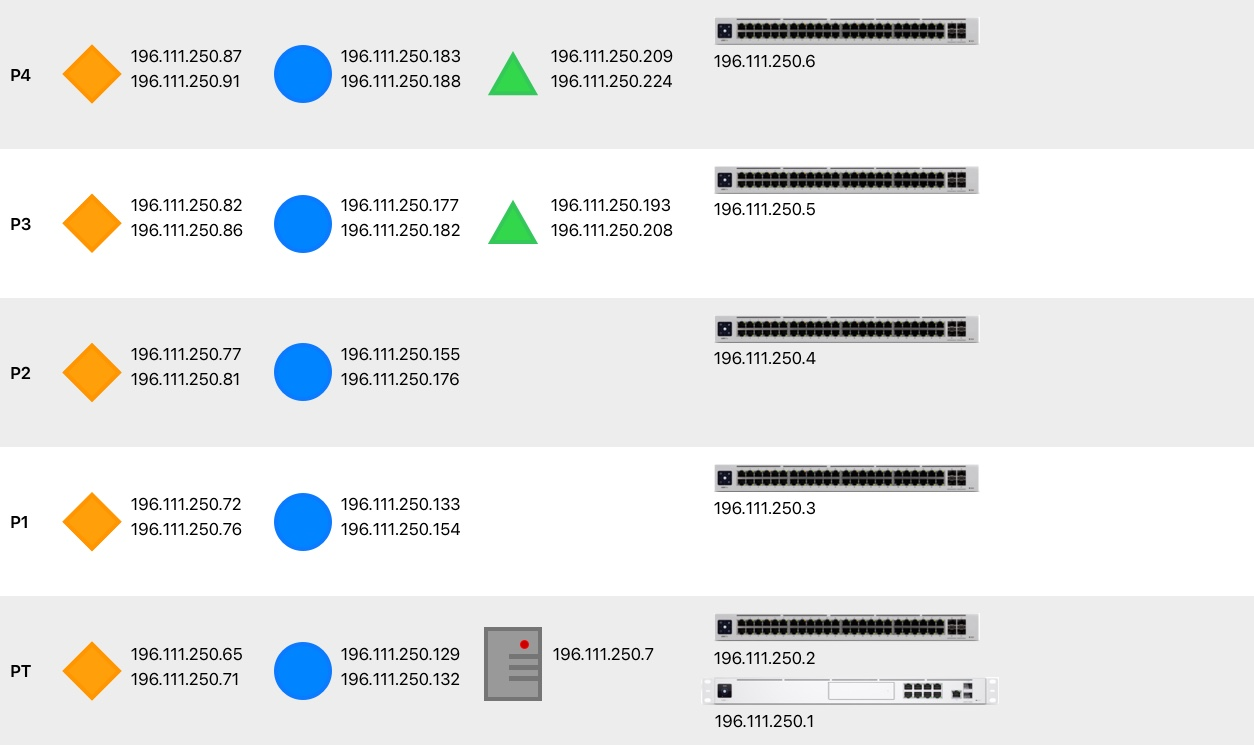
\includegraphics[width=\textwidth]{indirizzamento.jpg}
  \caption{Il piano di indirizzamento complessivo. Rombo: LAN amministrazione, cerchio: LAN produzione, triangolo: LAN sperimentale.}\label{fig:indirizzamento}
\end{figure}

Per eventuali server futuri aggiuntivi, si suppone che assumano degli indirizzi IP sequenziali rispetto al primo.

La soluzione presentata, in cui ogni postazione assume un indirizzo IP pubblico, richiede una particolare attenzione
dal punto di vista della sicurezza. Occorrerà impostare il gateway (il quale implementa funzionalità di sicurezza) in modo
da filtrare eventuali connessioni rischiose dall'esterno, come potenziali attacchi. Potrebbero essere necessari dei dispositivi
aggiuntivi, ma questo è al di fuori dello scopo di questa relazione.

La soluzione si presenta molto comoda nel caso in cui sia necessario avere accesso da remoto a tutte le macchine, si pensi ad esempio
alla semplicità con cui si può ricevere assistenza oppure accedere a computer ed altre strumentazioni anche lavorando da casa o fuori sede.          % INCLUDE: 3 - project

% --------------------------
% Back matter
% --------------------------
%
{%
    \setstretch{1.1}
    \renewcommand{\bibfont}{\normalfont\small}
    \setlength{\biblabelsep}{0pt}
    \setlength{\bibitemsep}{0.5\baselineskip plus 0.5\baselineskip}
    \printbibliography[nottype=online]
    \newrefcontext[labelprefix={@}]
    \printbibliography[heading=subbibliography,title={Webpages},type=online]
}

\cleardoublepage{}

\listoffigures
% \cleardoublepage{}

\listoftables
% \cleardoublepage{}

% \lstlistoflistings{}
% \cleardoublepage{}

% \appendix\cleardoublepage{}
% \input{content/chapters/appendix}       % INCLUDE: appendix

\cleardoublepage{}
% !TEX root = ../my-thesis.tex
%
\pagestyle{empty}
\hfill
\vfill
\pdfbookmark[0]{Colophon}{Colophon}
\section*{Colophon}

This thesis was typeset with \LaTeXe.
It uses the \textit{Clean Thesis} style developed by Ricardo Langner.
The design of the \textit{Clean Thesis} style is inspired by user guide documents from Apple Inc.

Download the \textit{Clean Thesis} style at \url{http://cleanthesis.der-ric.de/}.


% \cleardoublepage{}
% % !TEX root = ../my-thesis.tex
%
%************************************************
% Declaration
%************************************************
\pdfbookmark[0]{Declaration}{Declaration}
\addchap{Declaration}
\label{sec:declaration}
\thispagestyle{empty}

You can put your declaration here, to declare that you have completed your work solely and only with the help of the references you mentioned.

\bigskip

\noindent\textit{\thesisUniversityCity, \thesisDate}

\smallskip

\begin{flushright}
	\begin{minipage}{5cm}
		\rule{\textwidth}{1pt}
		\centering\thesisName
	\end{minipage}
\end{flushright}

%*****************************************
%*****************************************

% \clearpage

% \newpage
% \mbox{}

% **************************************************
% End of Document CONTENT
% **************************************************
\end{document}
